% !TeX root = index.tex
\iffalse
This chapter lays out your approach. 
What did you actually do to reach your goal, or attempt to reach your goal? 
What equipment did you use? 
How did you build the device? 
How did you set up the simulation: what mesh values, for example, did you use?

Provide enough detail that your work can be duplicated by someone else.
Be precise and use the correct units.
\fi


This section describes methods and design choices used to construct two processors.

\subsection{Machine Code}\label{subsec:machine_code}

\subsubsection{RISC}
As the aim of instruction size to be as minimal as possible, RISC instruction decided to be 8bits with optional additional immediate value from 1 to 3 bytes. Immediate values are explained in section \ref{subsec:imm_values}.

Decision was made to have instruction compose of operation code two operands - source/destination and source, which is similar to x86 architecture rather than MIPS. Three possible combinations of register address sizes are possible in such case from one to three bits. Two was selected as it allow having four general purpose registers which is sufficient for most applications, and allow four bits for operation code - allowing up to 16 instructions. 

Due to small amount of available operation codes and not all instructions requiring two operands (for example \texttt{JUMP} instruction may not need any operands or could use one operand to have address offset), other two type instructions are added to the design - with one and zero operands. See figure \ref{fig:risc_machinecode}. This enabled processor to have 45 different instructions while maintaining minimal instruction size. Final design has:
\begin{description}[labelindent=1cm, labelsep=1em]
	\item[$\bullet$ \textbf{8 }]  2-operand instructions
	\item[$\bullet$ \textbf{32}]  1-operand instructions
	\item[$\bullet$ \textbf{5 }]  0-operand instructions
\end{description}
Full list of RISC instructions are listed in table \ref{tab:risc_instructions} in \nameref{sec:appendix} section.

\begin{blockpage}
\begin{gather*}
\scalebox{0.8}{2 operands:}~
\underbrace{
	\colorbox{c1}{0}\,
	\colorbox{c1}{1}\,
	\colorbox{c1}{2}\,
	\colorbox{c1}{3}
}_\text{op. code}
\underbrace{
	\colorbox{c2}{4}\,
	\colorbox{c2}{5}
}_\text{dst.}
\underbrace{
	\colorbox{c3}{6}\,
	\colorbox{c3}{7}
}_\text{src.}
\\
\scalebox{0.8}{1 operand:}~
\underbrace{
	\colorbox{c1}{0}\,
	\colorbox{c1}{1}\,
	\colorbox{c1}{2}\,
	\colorbox{c1}{3}
}_\text{op. code}
\underbrace{
	\colorbox{c2}{4}\,
	\colorbox{c2}{5}
}_\text{dst.}
\underbrace{
	\colorbox{c1}{6}\,
	\colorbox{c1}{7}
}_\text{op. c.}\\
\scalebox{0.8}{0 operands:}~
\underbrace{
	\colorbox{c1}{0}\,
	\colorbox{c1}{1}\,
	\colorbox{c1}{2}\,
	\colorbox{c1}{3}\,
	\colorbox{c1}{4}\,
	\colorbox{c1}{5}\,
	\colorbox{c1}{6}\,
	\colorbox{c1}{7}
}_\text{operation code}
\end{gather*}
\begin{center}
\captionof{figure}{\textit{RISC instructions composition. Number inside box represents bit index. Destination (dst.) bits represents of source and destination register address.}}
\label{fig:risc_machinecode}
\end{center}
\end{blockpage}

\subsubsection{OISC}

As OISC requires only a single instruction, composition of instruction mainly requires two parts - source and destination. To allow higher instruction flexibility a immediate bit has been added to replace source address by immediate value. Composition of finalised machine code is shown in figure \ref{fig:oisc_machinecode}. 

\begin{blockpage}
\begin{gather*}
\underbrace{
	\colorbox{c1}{0}
}_\text{imm.}
\underbrace{
	\colorbox{c2}{1}\,
	\colorbox{c2}{2}\,
	\colorbox{c2}{3}\,
	\colorbox{c2}{4}\,
}_\text{destination}
\underbrace{
	\colorbox{c3}{5}\,
	\colorbox{c3}{6}\,
	\colorbox{c3}{7}\,
	\colorbox{c3}{8}\,
	\colorbox{c3}{9}\,
	\colorbox{c3}{10}\,
	\colorbox{c3}{11}\,
	\colorbox{c3}{12}
}_\text{source}
\end{gather*}

\begin{center}
\captionof{figure}{\textit{OISC instruction composition. Number inside box represents bit index.}}
\label{fig:oisc_machinecode}
\end{center}
\end{blockpage}

Decision was made to have source address to be eight bits to allow it be replaced with immediate value. Destination address was chosen to be as minimal as possible, leaving only four bits or 16 possible destinations. Final design has \textbf{15} destination and \textbf{41} source addresses. This is not the most space efficient design as 41 source addresses would require only six bits for address, wasting two bits every time non-immediate source is used.

Full list of OISC sources and destinations are listed in table \ref{tab:oisc_instructions} in \nameref{sec:appendix} section.
\subsection{Arithmetic Logic Unit}\label{subsec:alu}

\begin{figure*}[b]
\centering
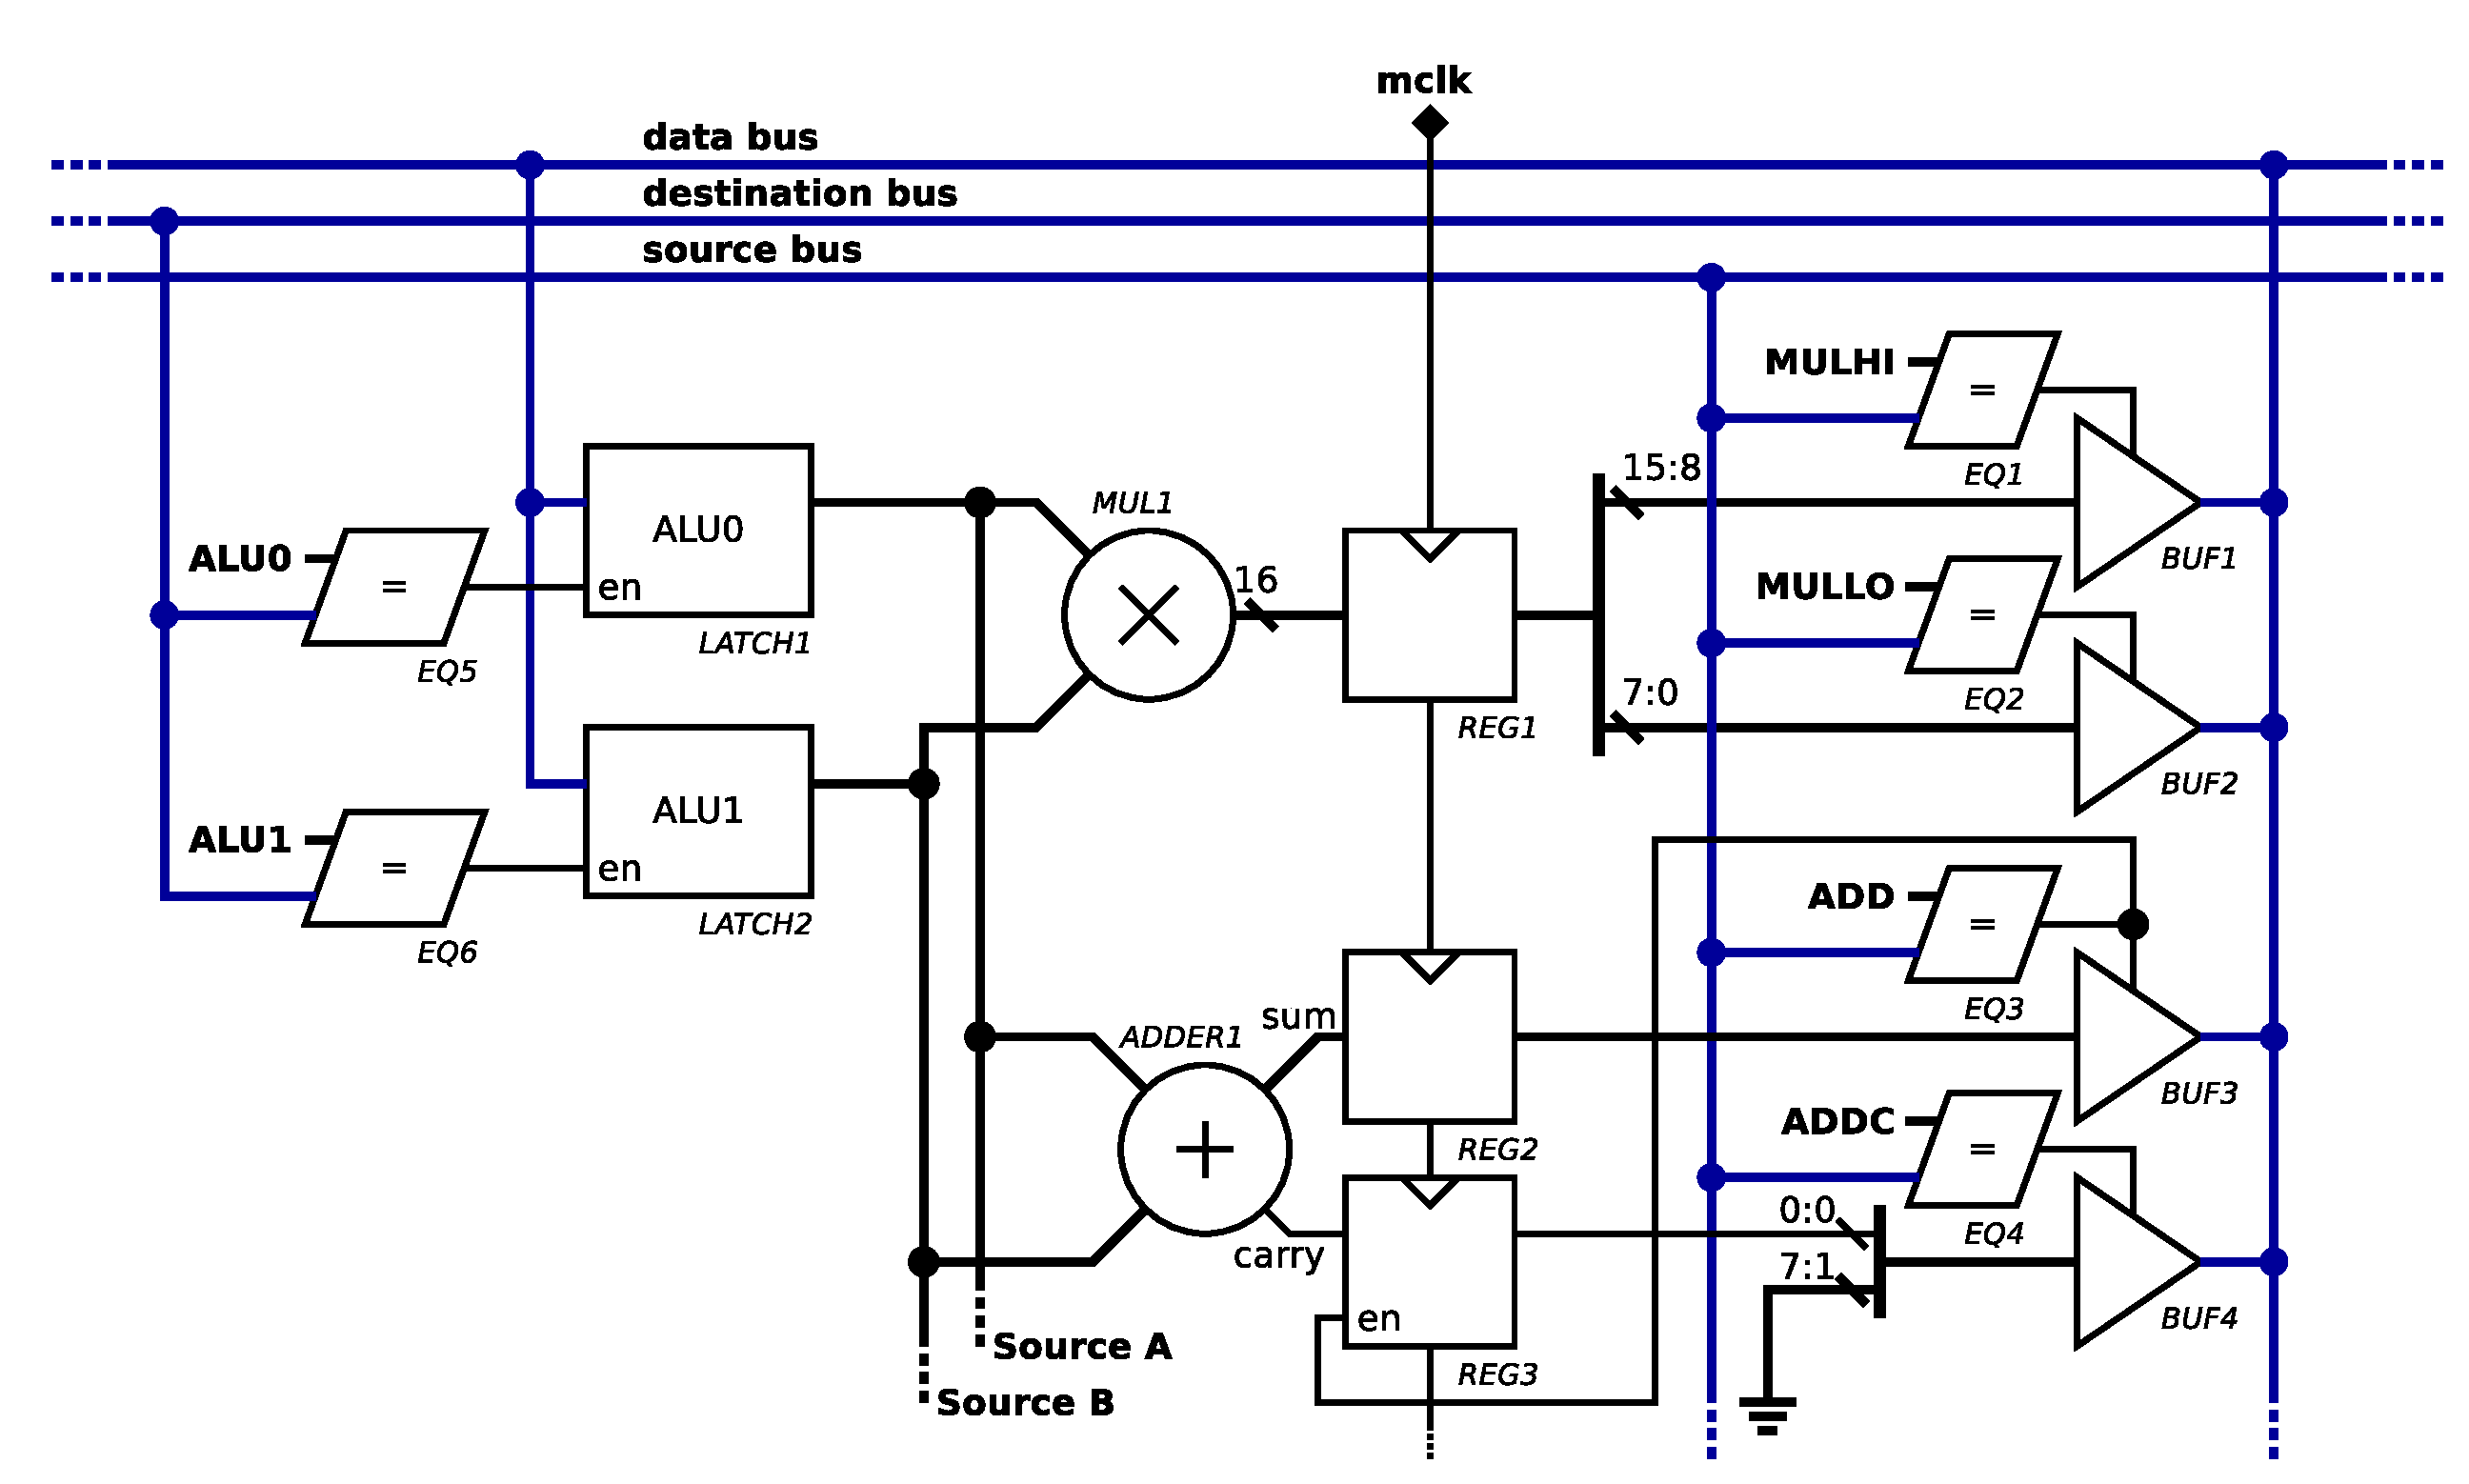
\includegraphics[scale=0.35]{../resources/oisc_alu.eps}
\caption{Digital diagram of OISC partial ALU logic}
\label{fig:oisc_alu}
\end{figure*}

This section will discuss ALU implementations of both processors. For fair comparison between OISC and RISC, ALU in both system will have the same capabilities described in table \ref{tab:alu_set}.

\begin{blockpage}
	\arrayrulecolor{black}
	\begin{tabular}{| c | p{0.75\linewidth} |} \hline 
		\rowcolor[rgb]{0.82,0.82,0.82}
		Name & Description \\\hline
		\arrayrulecolor[rgb]{0.82,0.82,0.82}
		ADD & Arithmetic addition (inc. carry) \\\hline
		SUB & Arithmetic subtraction (inc. carry) \\\hline
		AND & Bitwise AND \\\hline
		OR  & Bitwise OR \\\hline
		XOR & Bitwise XOR \\\hline
		SLL & Shift left logical \\\hline
		SRL & Shift right logical \\\hline
		ROL & Shifted carry from previous SLL \\\hline
		ROR & Shifted carry from previous SRL \\\hline
		MUL & Arithmetic multiplication \\\hline
		DIV & Arithmetic division \\\hline
		MOD & Arithmetic modulus \\
		\arrayrulecolor[rgb]{0,0,0}\hline
	\end{tabular}
	\captionof{table}{\textit{Supported ALU commands for both processors}}
	\label{tab:alu_set}
\end{blockpage}

\subsubsection{OISC}
Due to the structure of OISC processor, ALU source A and B are two latches that are written into when \texttt{ALU0} or \texttt{ALU1} destination address is present. ALU sources are connected with every ALU operator and performed in single clock cycle. This value is stored in register so that it would immediately available in a next clock cycle as a source data. Figure \ref{fig:oisc_alu} represents logic diagram of ALU with only addition and multiplication operators present. Note that output of \textit{EQ3} is connected to enable of \textit{REG3}, enabling output of carry to be only read after \texttt{ADD} source is requested. This previous source memory is also used for \texttt{SUB}, \texttt{ROL} and \texttt{ROR} operations. This allows processor to perform other operations such as store or load values, before accessing carry bit, or carried byte for \texttt{ROL} and \texttt{ROR} operations.

\subsubsection{RISC}
RISC processor has very similar structure to OISC with two exceptions. Inputs to ALU comes from logic router that decided how to route data in datapath. Output buffers are replaced by one multiplexer that selects single output from all ALU operations. Another point is that RISC ALU output is 16bit, higher byte saved in "ALU high byte register" for \texttt{MUL}, \texttt{MOD}, \texttt{ROL} and \texttt{ROR} operations. This register is accessible with \texttt{GETAH} instruction.

\subsection{Memory}\label{subsec:memory}
This section describes how instruction memory (ROM) is implemented for both processors.

\begin{figure*}[b]
	\centering
	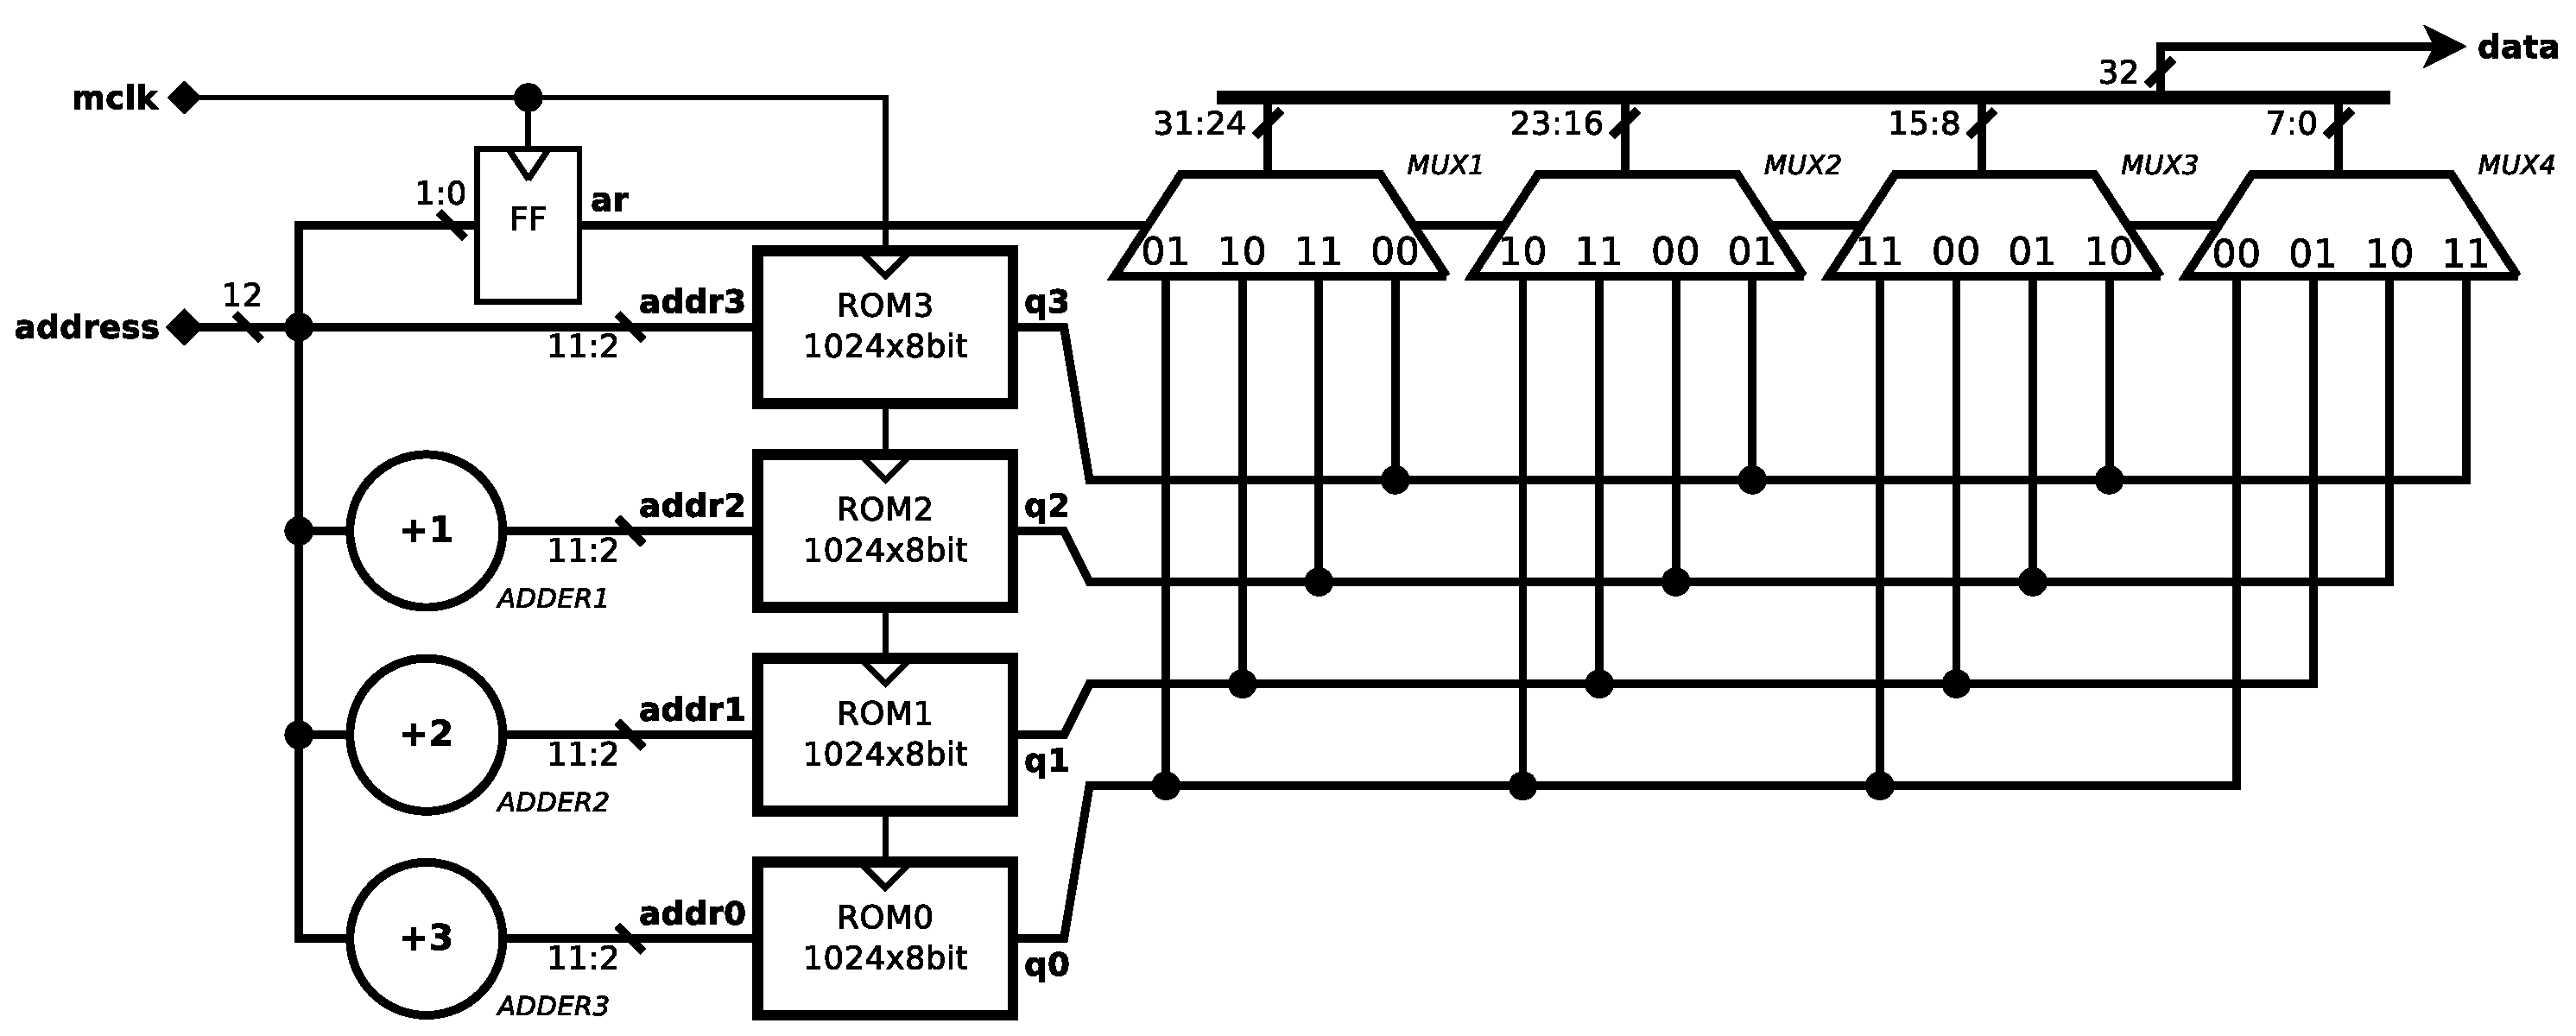
\includegraphics[scale=0.35]{../resources/risc_mem.eps}
	\caption{Digital diagram of RISC sliced ROM memory logic}
	\label{fig:risc_mem}
\end{figure*}

\subsubsection{RISC}
In order to allow dynamic instruction size from one to four bytes a special memory arrangement is made. A system was required to access word (8bits) from memory and next three words. To achieve this four ROM blocks been utilised, each containing one fourth of sliced original data. Input address is offset by adders \textit{ADDER1-3} and further divided by four by removing two least significant bits at \textbf{addr0-3}. 
Before concatenating output of each ROM block into final four bytes, ROM outputs \textbf{q0-3} are rearranged depending on \textbf{ar} signal. Note that \textit{MUX1-4} each input is different, this may be better visualised with Verilog code in listing \ref{code:rom_switch}.



\begin{blockpage}
\begin{lstlisting}[frame=single, language=Verilog, caption={RISC sliced ROM memory multiplexer arrangement Verilog code}, emph={ar, data}, label=code:rom_switch]
case(ar)
  2'b00: data={q3,q2,q1,q0};
  2'b01: data={q0,q3,q2,q1};
  2'b10: data={q1,q0,q3,q2};
  2'b11: data={q2,q1,q0,q3};
endcase
\end{lstlisting}
\end{blockpage}

\subsubsection{OISC}
OISC instructions are fixed 13 bits, which causes different problems to RISC sliced memory - non-standard memory word size. To implement ROM in FPGA, Altera Cyclone IV M9K memory configurable blocks were used. Each blocks as 9kB of memory each allowing 1024x9bit configuration. Combining three of such blocks together yields 27bits if readable data in single clock cycle. To store instruction code to such configuration, pairs of instruction machine code sliced into three parts plus one bit for parity check, see figure \ref{fig:oisc_memory_slice}. Circuit extracting each instruction is fairly simple, shown in figure \ref{fig:oisc_mem}.

\begin{figure*}[t]
\begin{gather*}
\overunderbraces{&\br{1}{ROM0}&\br{2}{ROM1}&\br{2}{ROM2}}%
{&
\colorbox{c1}{\scalebox{0.75}{00}}\,
\colorbox{c1}{\scalebox{0.75}{01}}\,
\colorbox{c1}{\scalebox{0.75}{02}}\,
\colorbox{c1}{\scalebox{0.75}{03}}\,
\colorbox{c1}{\scalebox{0.75}{04}}\,
\colorbox{c1}{\scalebox{0.75}{05}}\,
\colorbox{c1}{\scalebox{0.75}{06}}\,
\colorbox{c1}{\scalebox{0.75}{07}}\,
\colorbox{c1}{\scalebox{0.75}{08}}\,&
\colorbox{c1}{\scalebox{0.75}{09}}\,
\colorbox{c1}{\scalebox{0.75}{10}}\,
\colorbox{c1}{\scalebox{0.75}{11}}\,
\colorbox{c1}{\scalebox{0.75}{12}}\,&
\colorbox{c2}{\scalebox{0.75}{13}}\,
\colorbox{c2}{\scalebox{0.75}{14}}\,
\colorbox{c2}{\scalebox{0.75}{15}}\,
\colorbox{c2}{\scalebox{0.75}{16}}\,
\colorbox{c2}{\scalebox{0.75}{17}}\,&
\colorbox{c2}{\scalebox{0.75}{18}}\,
\colorbox{c2}{\scalebox{0.75}{19}}\,
\colorbox{c2}{\scalebox{0.75}{20}}\,
\colorbox{c2}{\scalebox{0.75}{21}}\,
\colorbox{c2}{\scalebox{0.75}{22}}\,
\colorbox{c2}{\scalebox{0.75}{23}}\,
\colorbox{c2}{\scalebox{0.75}{24}}\,
\colorbox{c2}{\scalebox{0.75}{25}}\,&
\colorbox{c3}{\scalebox{0.75}{26}}\,&
}%
{&\br{2}{InstrA}&\br{2}{InstrB}&\br{1}{parity}}
\end{gather*}
\caption{OISC three memory words composition. Number inside box represents bit index.}
\label{fig:oisc_memory_slice}
\end{figure*}

\begin{figure*}[t]
	\centering
	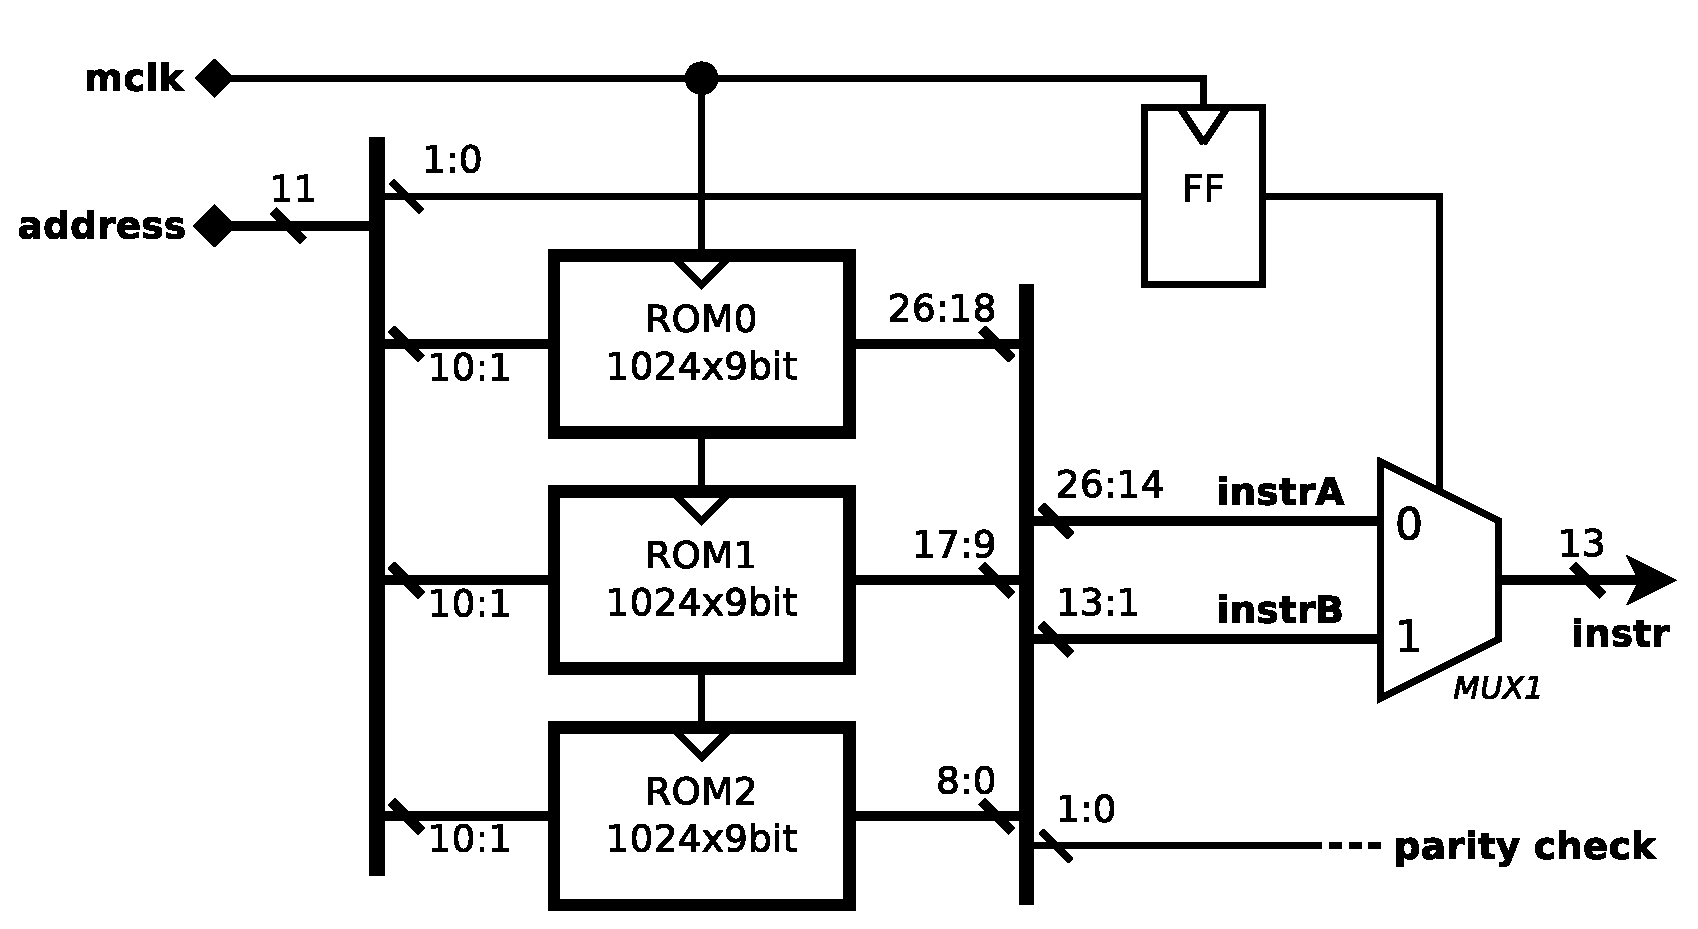
\includegraphics[scale=0.4]{../resources/oisc_mem.eps}
	\caption{Digital diagram of OISC instruction ROM logic}
	\label{fig:oisc_mem}
\end{figure*}

\subsection{Instruction decoding}\label{subsec:imm_values}
This section describes RISC and OISC differences between instruction decoding and immediate value handling.
\subsubsection{RISC}
Already described in previous section \ref{subsec:memory}, instruction from memory comes as 4 bytes. Least significant byte is sent to control block, other three bytes are sent to immediate override block (IMO) shown in figure \ref{fig:risc_imo}. These three bytes are labelled as \textbf{immr}. 


IMO block is a solution to change immediate value which enabled dynamically calculated memory pointers, branches dependant on register value or any other function that needs instruction immediate value been replaced by calculated register value. IMO is controlled by control block and \textbf{cdi.imoctl} signal, which is changed by \texttt{CI0}, \texttt{CI1} and \texttt{CI2} instructions. When signal is \texttt{0h}, this block is transparent connecting \textbf{immr} directly to \textbf{imm}. When any of \texttt{CI} instructions executed, one of IMO register is overridden by \textit{reg1} value from register file. In order to override two or three bytes of immediate, \texttt{CI} instructions need to be executed in order. Only for one next instruction after last \texttt{CI} will have immediate bytes changed depending on what are values in \textit{IMO} registers.
\\This circuit has two disadvantages: 
\begin{enumerate}
	\item Overriding immediate bytes takes one or more clock cycles,
	\item At override, \textbf{immr} bytes are ignored therefore they are wasting instruction memory space.
\end{enumerate}
Second point can be resolved by designing a circuit that would subtract the amount of overridden IMO bytes from \textit{pc\_off} signal (program counter offset that is dependant on i-size value) at the program counter, thus effectively saving instruction memory space. This solution however would introduce a complication with the assembler as additional checks would need to be done during compiling to check if IMO instruction are used.

\begin{figure*}[t]
	\centering
	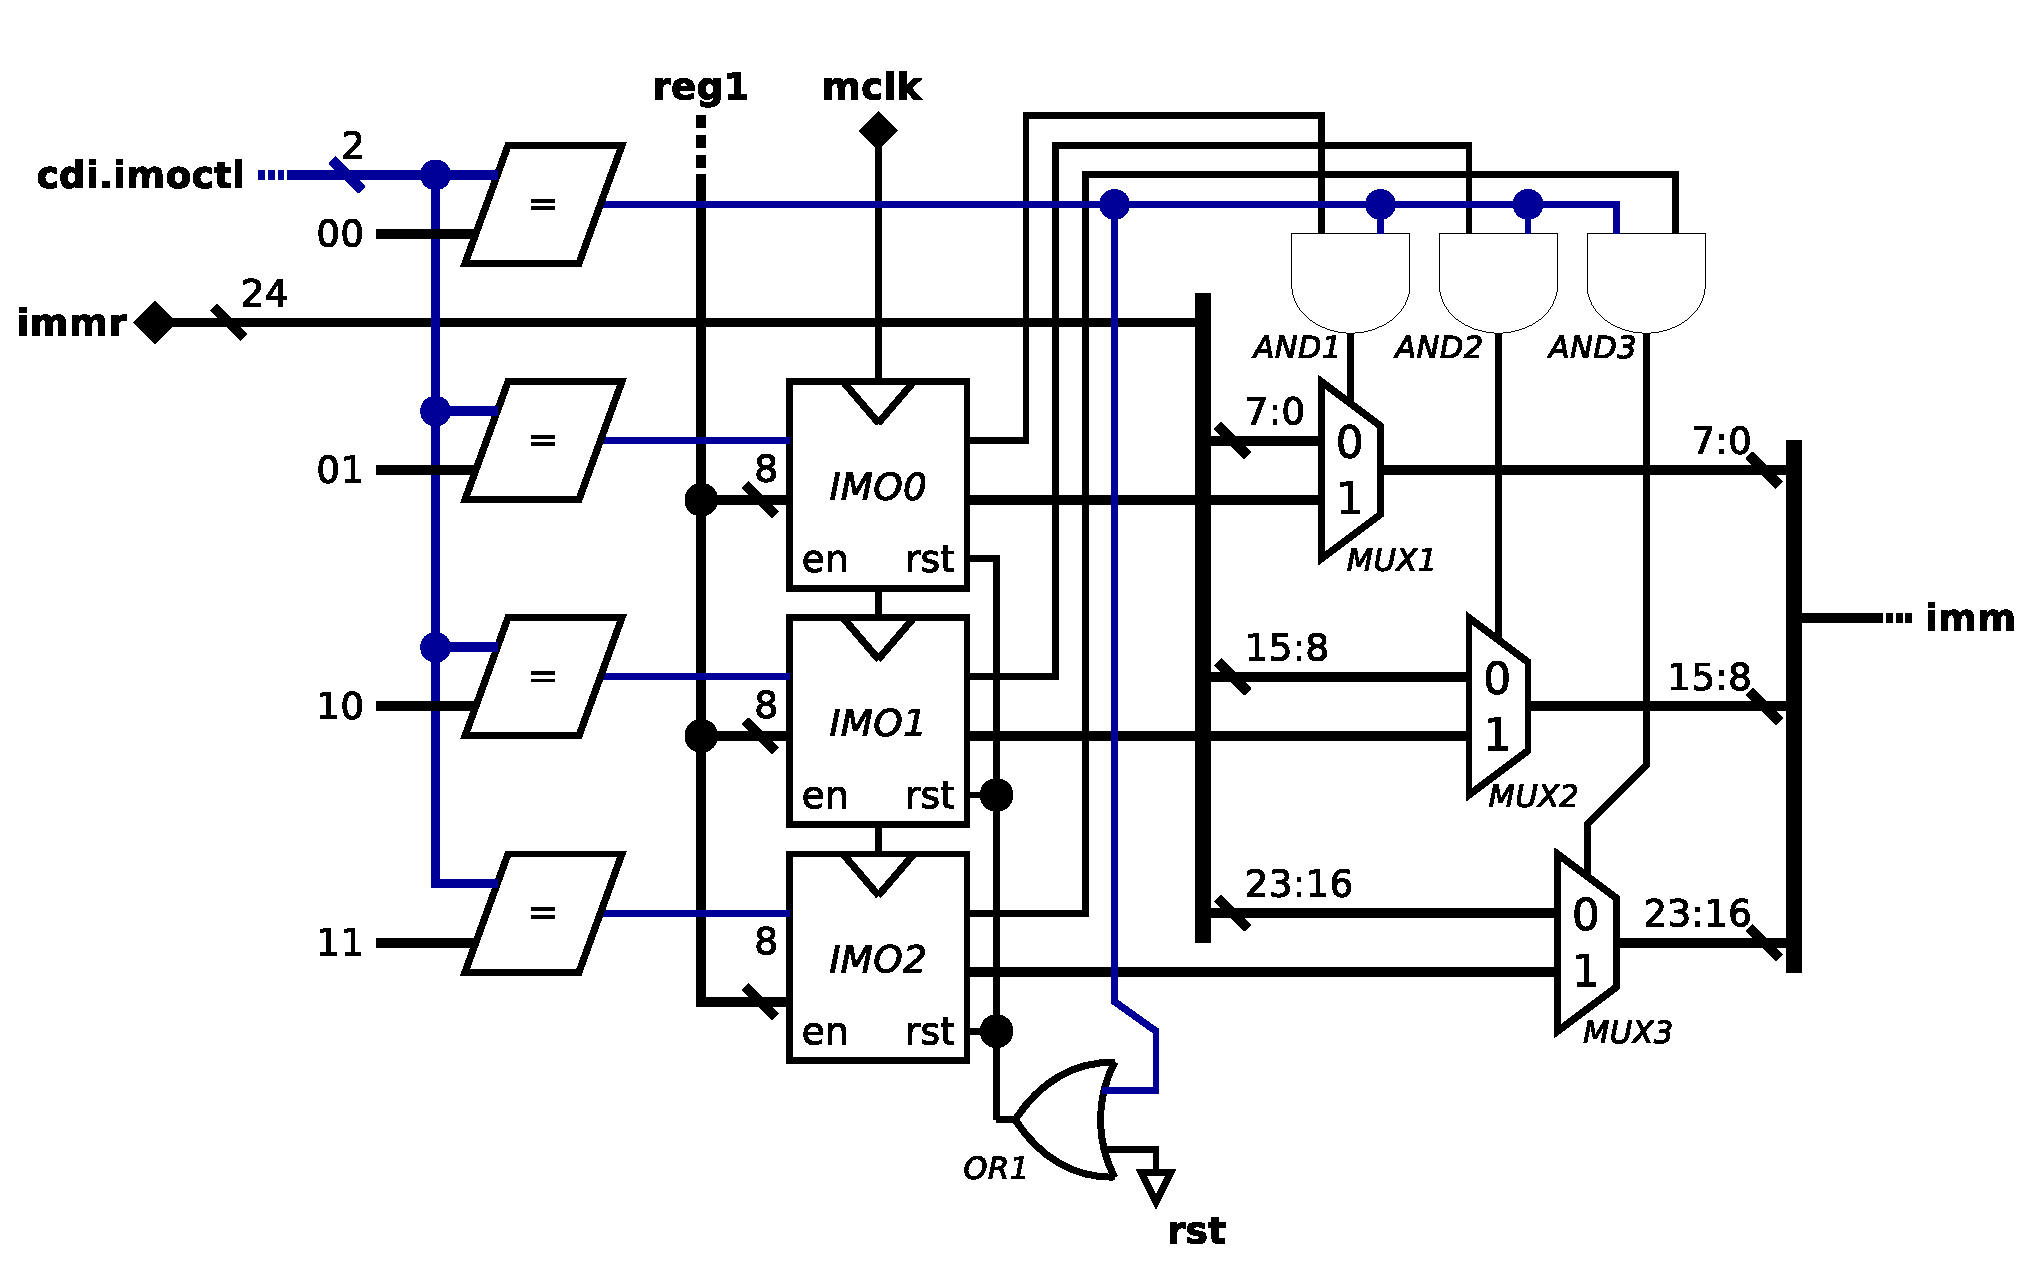
\includegraphics[scale=0.4]{../resources/risc_imo.eps}
	\caption{Digital diagram of RISC immediate override system}
	\label{fig:risc_imo}
\end{figure*}

\begin{figure*}[t]
	\centering
	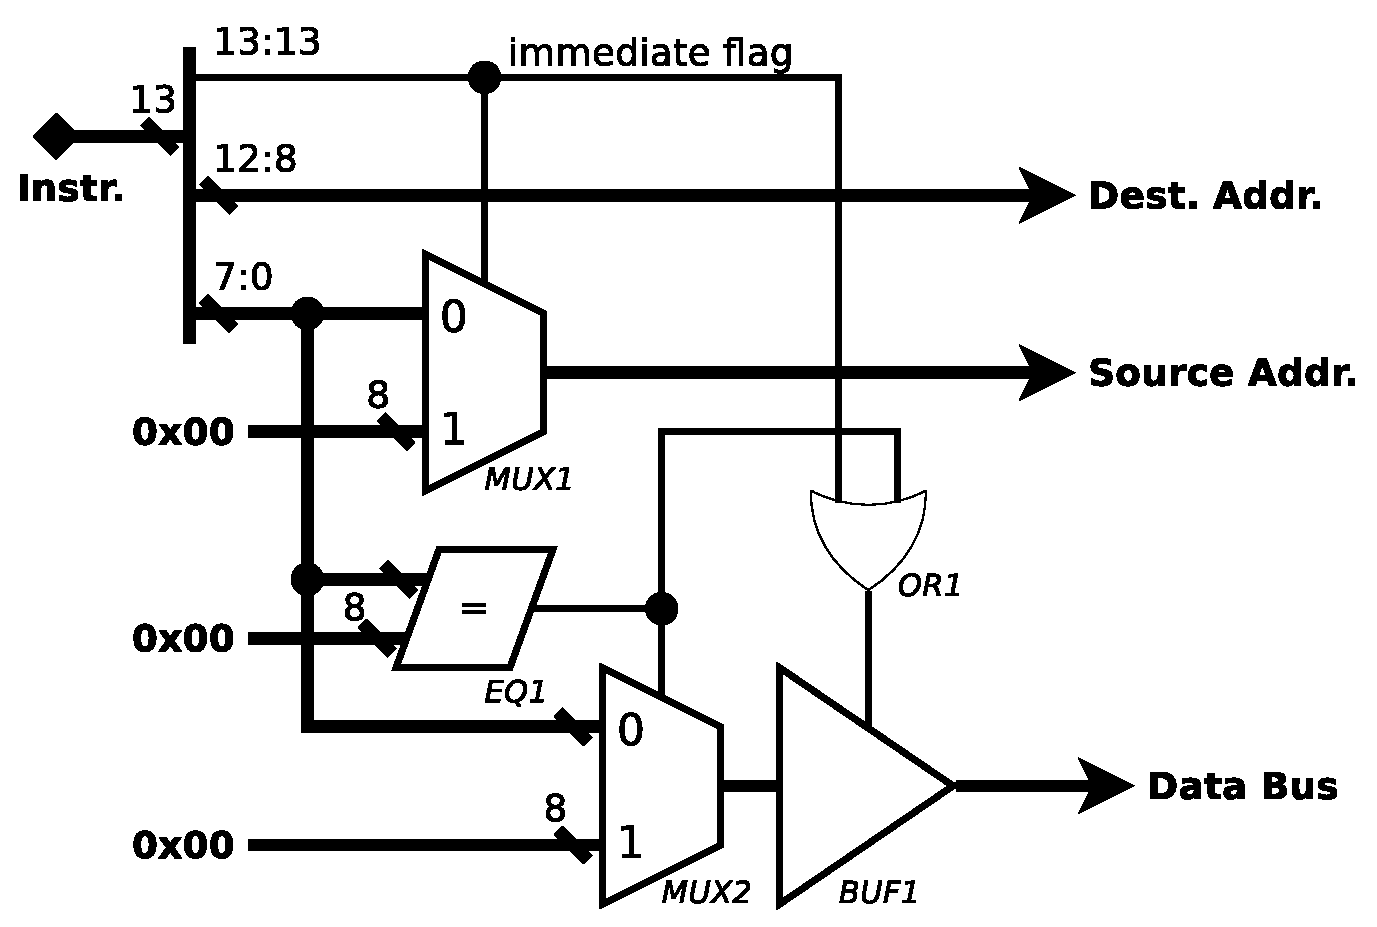
\includegraphics[scale=0.4]{../resources/oisc_decoder.eps}
	\caption{Digital diagram of OISC instruction decoder}
	\label{fig:oisc_decoder}
\end{figure*}

\subsubsection{OISC}
OISC immediate value is set in instruction decoder shown in figure \ref{fig:oisc_decoder}. Decoder operation is simple - instruction machine code is split into three parts as described in \ref{fig:oisc_machinecode}. If instruction source address is \texttt{00h}, connect data bus with constant 0 via \textit{MUX2}. If immediate bit is 1, set source address to \texttt{00h} (to make sure no other buffer source connects to data bus), and connect instruction source address (immediate value) to databus via \textit{MUX2} and \textit{BUF1}. 





